\section{Présentation du projet \gls{OPEROSE}}
\paragraph{}
L’équipe COPAIN, dont j’ai fait partie durant ma période de stage, de l’unité TSCF, participe à l’organisation opérationnelle du Challenge \gls{ANR} \gls{ROSE}. Ce dernier, a pour objectif d’encourager le développement de solutions innovantes autonomes en matières de désherbages intra-rang de grandes cultures à fort écartement (ex maïs, tournesol, …) et des cultures légumières de plein champ afin de réduire l’usage des herbicides. En effet, des solutions technologiques existent pour éliminer les mauvaises herbes entre deux rangs de cultures(l’inter-rang) sans utiliser des produits chimiques, mais peu d’alternatives sont proposées pour le désherbage de l’intra-rang, c’est-à-dire entre les plants d’un même rang. C’est ainsi que le ministère chargé de l’Agriculture et de la Transition Écologique en partenariat avec le ministère de la Recherché et l’ANR, dans le cadre du plan Ecophyto II, ont lancé le challenge ROSE.  Ce Challenge a débuté en janvier 2018 et durera quatre ans, durant lesquelles, quatre campagnes d’évaluations seront menées par le consortium en charge de l’organisation à savoir IRSTEA/LNE avec la participation de VetAgro Sup.  
\paragraph{}
L’avancée des travaux sera mesurée tout au long du projet lors de rencontres annuelles sur le terrain durant lesquelles les chercheurs réaliseront certaines tâches précises, dans un cadre de répétabilité et de reproductibilité des expériences menées. Les confrontations seront organisées selon une procédure élaborée en concertation avec les chercheurs, par le LNE/IRSTEA. 

\begin {figure}[!h]
\begin{center}

    \hbox{ 
    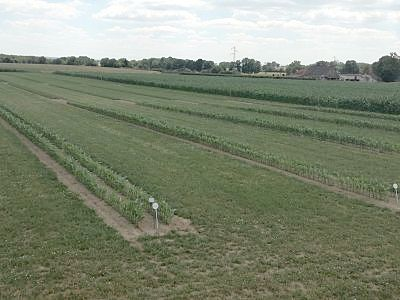
\includegraphics[width=5cm]{images/imageRang1.jpg}
    \hspace*{1cm}  %% pour mettre un espace (horizontal) de 5cm entre les deux images
    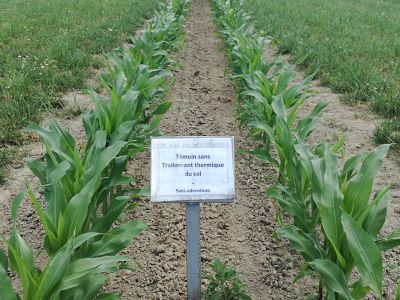
\includegraphics[width=5cm]{images/imageRang2.jpg}
  }
\caption{Rangées de cultures pour le challenge Rose}
\label{Rangées de cultures pour le challenge Rose}
\end{center}
\end {figure}

\url{http://challenge-rose.fr/}


